\section{Betriebssysteme}

\subsection{Grundlagen}

\subsubsection{Definition Betriebssystem (Operating System)}
Ein Betriebssystem stellt das Bindeglied zwischen der Hardware eines Computers einerseits und dem Anwender bzw. seinen Programmen andererseits dar. Es umfasst Programme, die zusammen mit den Eigenschaften des Computers die Grundlage der möglichen Betriebsarten dieses Systems bilden und insbesondere die Abwicklung von Programmen steuern und überwachen.

\subsubsection{Virtuelle Maschine (Virtual Machine)}
Das Betriebssystem wird gelegentlich auch als Virtuelle Maschine bezeichnet. Die beiden Begriffe dürfen aber nicht einfach gleichgesetzt werden, da sie sich von der Definition her klar unterscheiden. \\
Unter dem Begriff "Virtuelle Maschine" versteht man einfach gesagt Software, die vorgibt, ein eigenständiger Rechner zu sein. Man kann es sich so vorstellen, als ob man neben einem Computer einen weiteren aufstellt – mit dem Vorteil, dass man mit wenigen Mausklicks zwischen verschiedenen Betriebsystemen hin- und herwechseln kann.\\\\
\textbf{Formen und Ausprägungen virtueller Maschinen:}
\begin{itemize}
    \item Hardware + Laufzeitumgebung des Sprachsystems
    \begin{itemize}
        \item Geeignet für Kleinsysteme mit einfacher Peripherie.
        \item Bereitgestellt werden Dienste zur Programmausführung, eventuell angereichert für die Parallelverarbeitung durch die Laufzeitbibliothek (z.B. C++ oder Java).
    \end{itemize}
    \item Hardware + Betriebssystem
    \begin{itemize}
        \item Abgestuft im Funktionsumfang für Systeme jeder Grössenordnung geeignet.
        \item Bereitgestellt werden Ein/Ausgabedienste und Mittel zur Parallelverarbeitung (z.B. Linux, Windows-NT, einfache Betriebssysteme für Mikrokontroller).
    \end{itemize}
\end{itemize}

\subsubsection{Schichtenmodell des Computersystems}
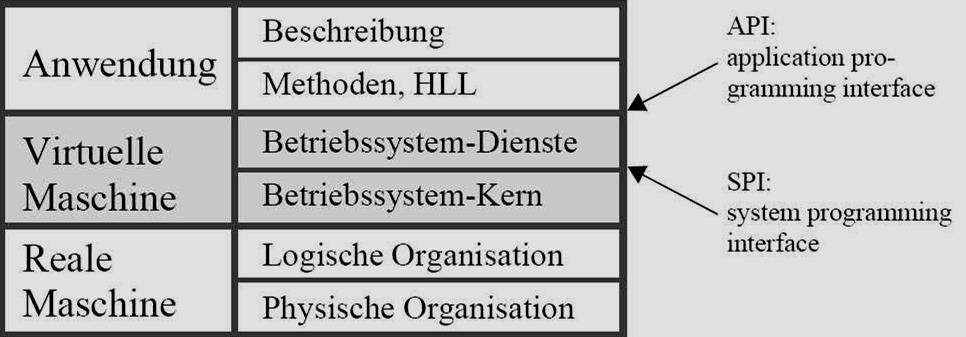
\includegraphics[width=0.3\textwidth]{images/Betriebssysteme/Schichtenmodell.png}\\
Das Betriebssystem im Schichtenmodell des Computersystems
\begin{itemize}
    \item bietet der Anwendung API-Schnittstellen (Schnittstelle zur Anwendungsprogrammierung) zur Realen Maschine
    \item macht die Anwendung damit weitgehend unabhängig von der Realen Maschine (CPU, Hardware, Peripherien,...)
\end{itemize}

\subsubsection{Schnittstellen}
Operating Systems verfügen in der Regel über vergleichbare Programmierstellen.
Oft werden zwei Schichten unterschieden:
\begin{itemize}
    \item Betriebssystem-Dienste: Höhere Funktionen des Betriebssystems, welche direkt von der Anwendung benutzt werden.
    \item Betriebssystem-Kern: Kernfunktionen des Betriebssystems wie Prozessverwaltung, Prozesssynchronisation, Interprozess-Kommunikation, Exception-und Interrupt-Handling, usw. Oft als Mikrokern (microkernel) realisiert.
\end{itemize}

\subsubsection{Anwenderprogramm ohne/mit Betriebssystem}
\begin{minipage}{0.5\textwidth}
    \textbf{Rechner ohne Betriebssystem:}\\
    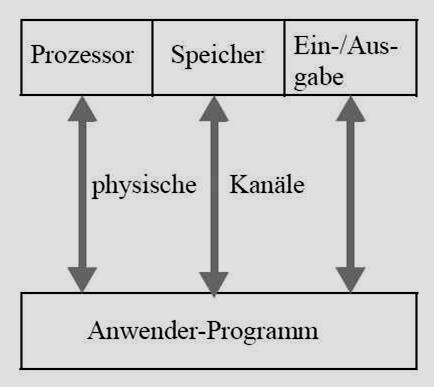
\includegraphics[width=0.6\textwidth]{images/Betriebssysteme/Rechner_ohne_Betriebssystem.png} \\
        Anwender-Programm greift direkt über physikalische Kanäle auf die Reale Maschine zu $\rightarrow$ ist eng mit der Realen Maschine gekoppelt \\ \\ \\ \\
\end{minipage}
\hfill
\begin{minipage}{0.45\textwidth}
    \textbf{Rechner mit Betriebssystem:}\\
    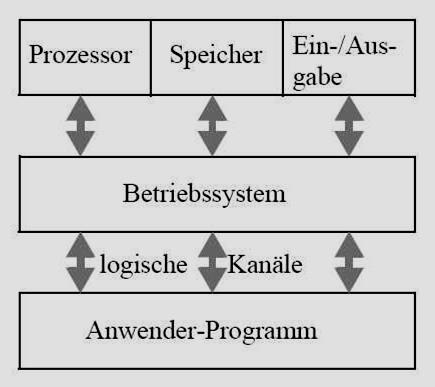
\includegraphics[width=0.7\textwidth]{images/Betriebssysteme/Rechner_mit_Betriebssystem.png} \\
        Das Betriebssystem bildet eine klare Abstraktionsschicht für den Zugriff auf die Reale Maschine $\rightarrow$ entkoppelt die Reale Maschine vom Anwender
        Bietet dem Anwender-Programm über logische Kanäle zusätzliche Funktionen, Möglichkeiten und Dienste an
\end{minipage}

\subsubsection{Kernfunktionen}
\begin{minipage}{0.5\textwidth}
    \begin{itemize}
        \item Parallele Prozesse
        \item Interprozess-Kommunikation
        \item Peripherie-und Geräte-Treiber
        \item Hardware-Abstraktion
    \end{itemize}
\end{minipage}
\hfill
\begin{minipage}{0.45\textwidth}
    \begin{itemize}
        \item Utility Funktionen
        \item Speicher-Management
        \item Dateisysteme
        \item etc.
    \end{itemize}
\end{minipage} \\ \\ \\
Betriebssysteme kommen insbesondere dann zur Anwendung, wenn die Laufzeitumgebung des Sprachsystems selbst keine oder zu geringe Möglichkeiten für die Parallelverarbeitung bietet.

\subsubsection{Architekturen}
\begin{minipage}{0.3\textwidth}
    \begin{itemize}
        \item Monolitische Architektur\\\\ 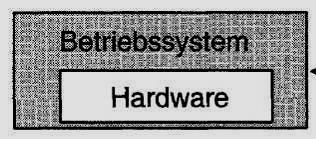
\includegraphics[width=0.6\textwidth]{images/Betriebssysteme/Monolitische_Architektur.png}
        \item Kern-Schale Architektur\\\\
        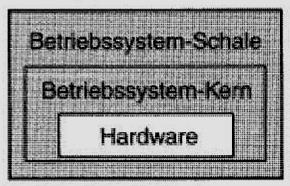
\includegraphics[width=0.6\textwidth]{images/Betriebssysteme/Kern-Schale_Architektur.png} \\ \\ \\ \\ \\ \\
    \end{itemize}
\end{minipage}
\hfill
\begin{minipage}{0.3\textwidth}        
    \begin{itemize}
        \item Hierarchische Schichten\\\\
        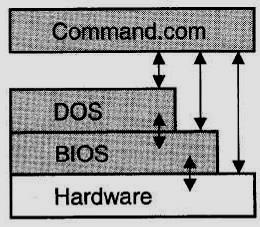
\includegraphics[width=0.6\textwidth]{images/Betriebssysteme/Hierarchische_Schichten.png}
        \item Mikrokern\\\\
        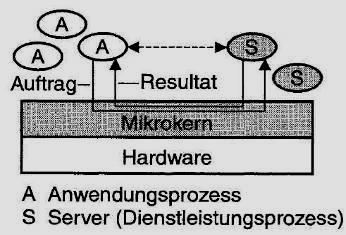
\includegraphics[width=0.6\textwidth]{images/Betriebssysteme/Mikrokern.png} \\ \\ \\
    \end{itemize}
\end{minipage}
\hfill
\begin{minipage}{0.3\textwidth}
    \begin{itemize}
        \item Virtuelle Maschinen\\\\
        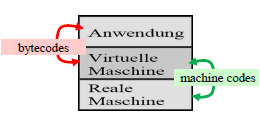
\includegraphics[width=0.8\textwidth]{images/Betriebssysteme/Virtuelle_Maschinen.png} \\ \\ \\ \\ \\ \\ \\ \\ \\ \\ \\ \\ \\
    \end{itemize}
\end{minipage}

\subsubsection{Klassifikation}
\textbf{Betriebsarten (operation mode):}
\begin{itemize}
    \item Stapelverarbeitung: Bearbeitung einer Folge von Stapelaufträgen. Jobs werden immer ohne Interaktion des Benutzers vollständig abgearbeitet.
    \item Dialogbetrieb:Ständiger Wechsel zwischen Aktionen des Benutzers und solchen des Systems. Benutzer kann den Arbeitsablauf im Dialog jederzeit beeinflussen.
    \item Echtzeitverarbeitung: Einsatz eines Computersystems zur Steuerung und Überwachung von technischen Prozessen. Die Einhaltung von Zeitbedingungen muss gesichert sein.
    \item Verteilte Verarbeitung:Das System besteht aus mehreren miteinander gekoppelten Computern. Das Betriebssystem dient vorrangig der Verteilung von Daten, Ressourcen und Arbeitslast.
\end{itemize}
\textbf{Anzahl der Benutzer (number of users):}
\begin{itemize}
    \item Einzelnutzer-System
    \item Mehrnutzer-System
\end{itemize}
\textbf{Anzahl der Aufträge (number of tasks):}
\begin{itemize}
    \item Einzelprozess-System: System kann jeweils nur einen einzigen Auftrag bearbeiten. Weitere Aufträge werden erst nach Beendigung des aktuellen Auftrages angenommen. 
    \item Mehrprozess-System: Kann gleichzeitig mehrere verschiedene Aufträge verwalten und parallel oder zumindest quasi-parallel bearbeiten.
\end{itemize}

\subsubsection{Hauptkomponenten und Entwurfskriterien}
\textbf{Hauptkomponenten:}\\ \\
\begin{minipage}{0.5\textwidth}
    \begin{itemize}
        \item Prozessverwaltung und -koordinierung 
        \item Interprozess-Kommunikation
        \item Ein-/Ausgabe-Steuerung
        \item Kommunikation mit der Umgebung
        \item Auftragsverwaltung
        \item Benutzerverwaltung
    \end{itemize}
\end{minipage}
\hfill
\begin{minipage}{0.45\textwidth}
    \begin{itemize}
        \item Betriebsmittelverwaltung
        \item (Haupt-) Speicherverwaltung
        \item Dateiverwaltung
        \item Benutzerunterstützung
        \item etc.
    \end{itemize}
\end{minipage} \\ \\ \\
\textbf{Entwurfskriterien:}\\ \\
\begin{minipage}{0.5\textwidth}
    \begin{itemize}
        \item Modularität und Orthogonalität
        \item inkrementelle Erweiterbarkeit und Konsistenz
        \item statische oder dynamische Konfigurierung, Rekonfigurierung
        \item Skalierbarkeit
    \end{itemize}
\end{minipage}
\hfill    
\begin{minipage}{0.45\textwidth}
    \begin{itemize}
        \item Zuverlässigkeit und Fehlertoleranz
        \item Portierbarkeit
        \item Transparenz und Virtualisierung
        \item etc.
    \end{itemize}
\end{minipage}

\subsubsection{Benutzerschnittstelle}
Neben den funktionalen API-Schnittstellen werden oft auch User Interfaces bereitgestellt. Dabei wird mit Hilfe eines Kommando-Interpreters oder einer grafischen Benutzeroberfläche die Bedienanforderungen ausgewertet.


\subsection{Multitasking}

\subsubsection{Parallelverarbeitung}
\begin{minipage}{0.5\textwidth}
    Eine Parallelverarbeitung liegt dann vor, wenn verschiedene Programme oder Programmteile gleichzeitig bearbeitet werden. Anwendungsabhängig besteht oft die Notwendigkeit zwischen einzelnen Prozessen Informationen auszutauschen. Diese Art von Prozessen werden als parallele, miteinander kooperierende Prozesse bezeichnet. \\ \\
    \textbf{Quasi-Parallelität:} Verfahren, das erlaubt mehrere Prozesse auf einem Prozessor auszuführen.\\ \\
    \textbf{Nebenläufige Prozesse:} Wird benutzt um die quasi-parallele Ausführung auf einem Einprozessor-System zu bezeichnen\\ \\
    \textbf{Task:} Alternative Bezeichnung zu Prozess
\end{minipage}
\hfill
\begin{minipage}{0.45\textwidth}
    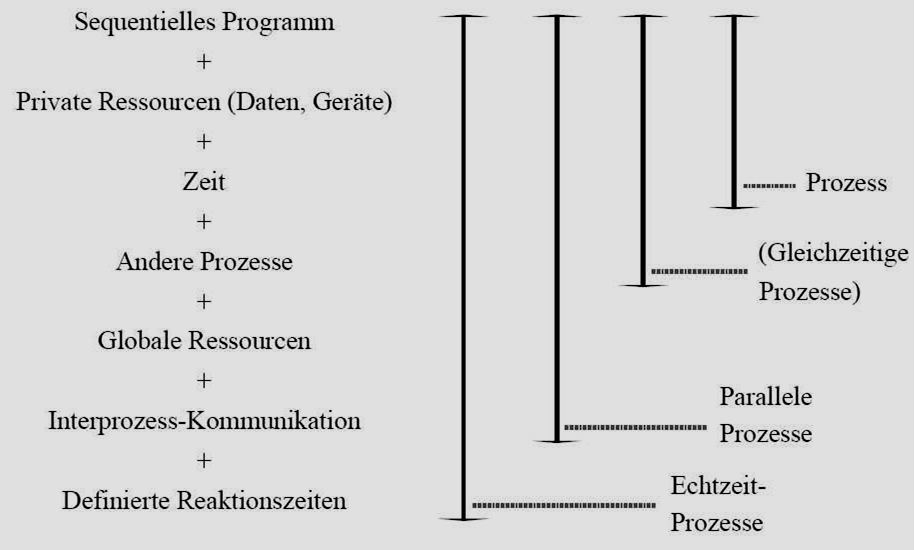
\includegraphics[width=1.0\textwidth]{images/Betriebssysteme/Parallelverarbeitung.png}
\end{minipage}
	
\subsubsection{Parallele Prozesse}
\begin{minipage}{0.5\textwidth}
    Im Schichtenmodell können parallele Prozesse auf der Anwendungsebene, der virtuellen Ebene und der physischen Ebene betrachtet werden. Es kann jedoch vorkommen, dass die parallelen Prozesse auf der Anwendungsebene nicht notwendigerweise 1:1 auf die Prozesse der virtuellen Maschine abgebildet werden. \\ \\
    Nebst Anwendungsprozessen gibt es auch dauernd existierende Betriebssystemprozesse im Hintergrund. Man nennt sie Dämonen. 
\end{minipage}
\hfill
\begin{minipage}{0.45\textwidth}
    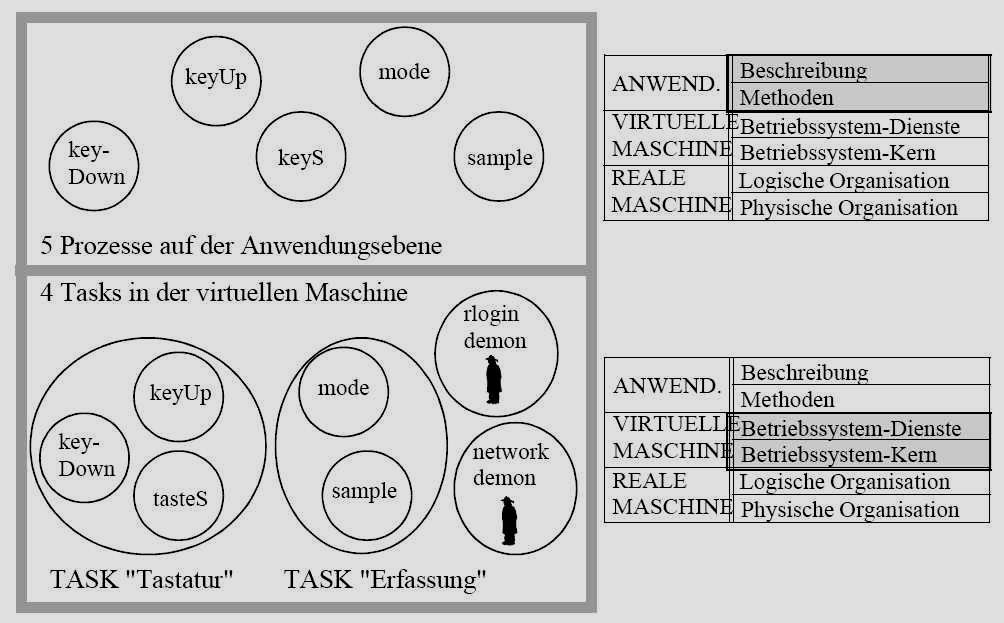
\includegraphics[width=1.0\textwidth]{images/Betriebssysteme/ProzesseAufVerschEbenen.png}
\end{minipage} \\ \\ \\
Je nach Betriebsumgebung werden abweichende Begriffe für Prozesse verwendet (Jobs/Sessions, Prozesse/Tasks, Threads/Stränge/Fäden/Leichtgewichtsprozesse).

\subsubsection{Prozesszustände}
\begin{multicols}{2}
\begin{itemize}
    \item Inactive: Formaler Zustand für Prozesse, die noch nicht oder nicht mehr im System existieren
    \item Ready: Der Prozess wartet auf die Zuteilung eines Prozessors (keine weiteren Wartebedingungen). Sind mehrere Prozesse im Ready-Zustand, so entscheidet das Betriebssystem auf Grund seiner Abfertigungsstrategie, welcher in den Running -Zustand wechseln darf. 
    \item Running: Der Prozess hat den Prozessor zugeteilt bekommen und schreitet voran (er läuft).In einem Einprozessor-System kann maximal 1 Prozess in diesem Zustand sein.
    \item Waiting: Der Prozess wartet auf das Erfüllen von (mindestens) einer Wartebedingung.
\end{itemize} \ \ \ \ \
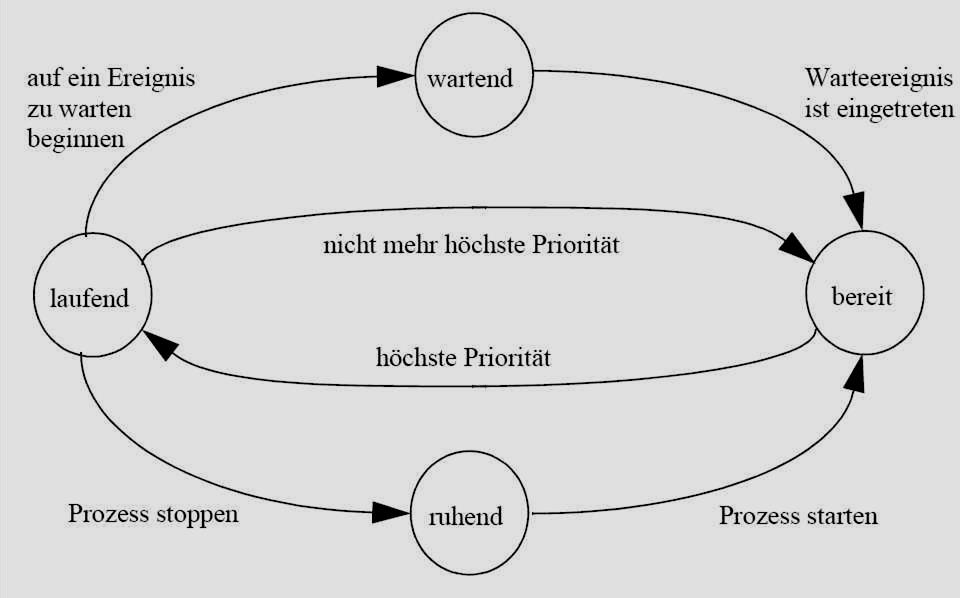
\includegraphics[width=0.4\textwidth]{images/Betriebssysteme/Prozesszustaende.png}
\end{multicols}
Das Betriebssystem verwaltet mehrere Listen:
\begin{itemize}
    \item ss: Enthält die lauffähigen Prozesse. Es können mehrere ssen vorhanden sein, z.B. eine für jede Prioritätsstufe.
    \item Waiting-Listen: für sämtliche unterscheidbaren Warte-Ereignisse wird eine eigene Waiting-List geführt.
\end{itemize}

\subsubsection{Scheduling und Context Switch}
\textbf{Context:} Zur Verwaltung im Betriebssystem besitzt jeder Prozess einen eigenen Kontext. Dieser enthält alle relevanten Informationen über den Prozess: 
\begin{itemize}
    \item Speicher-Kontext: Speicherabbild des Prozesses (Programm-Code, Stack, Daten)
    \item Hardware-Kontext: Registerabbild (Programcounter, Stackpointer, Registerinhalte, usw.)
    \item System-Kontext: Betriebssysteminterne Verwaltungsdaten zum Prozess (auch als TCB bezeichnet)
\end{itemize}
\textbf{Task Control Block (TCB):}
Wird die Datenstruktur, in welcher der Kontext der
Prozesse abgelegt werden kann, bezeichnet.\\\\
Ein \textbf{Prozesswechsel (task switch)} bedeutet:
\begin{itemize}
    \item Der aktive Prozess gibt den Prozessor entweder freiwillig ab oder er bekommt ihn entzogen. 
    \item Die Auswahl des Prozesses, dem der Prozessor als nächstes zugeteilt wird, erfolgt durch den Scheduler anhand einer vordefinierten Scheduling-Strategie.
    \item Ein Prozesswechsel (wird vom Dispatcher des OS gesteuert) kann i.d.R. nur mittels einer Unterbrechung stattfinden (HW-Unterbrechung/Interrupt oder SW-Unterbrechung/Systemdienstaufruf).
\end{itemize}
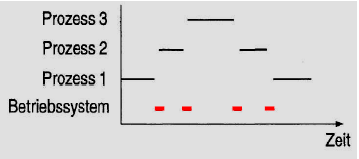
\includegraphics[width=0.3\textwidth]{images/Betriebssysteme/Prozesswechsel.png} \\\\
\textbf{Aktionen im OS bei Context Switch:}
\begin{enumerate}
    \item Sicherung des gesamten Kontextes des unterbrochenen Prozesses
    \item Änderung des Zustandes des unterbrochenen Prozesses in \textit{Ready} oder \textit{Waiting}, je nach Grund der Unterbrechung
    \item Auswahl des zu aktivierenden Prozesses durch den Scheduler
    \item Änderung des Zustandes des zu aktivierenden Prozesses von \textit{Ready} in \textit{Running}
    \item Wiederherstellung des (gesicherten) Kontextes dieses Prozesses. Durch Laden der Prozessorregister wird dieser Prozess fortgesetzt.
\end{enumerate}
\textbf{Idle Task:} Der Idle Task besteht meist nur aus einer Warteschleife, so dass er jederzeit
problemlos verdrängt werden kann. Er wird nur dann aktiv, wenn beim Scheduling kein anderer Prozess laufbereit ist. Ohne den Idle Task müsste innerhalb des Betriebssystem-Kerns gewartet werden
(busy waiting).\\\\
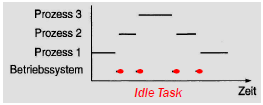
\includegraphics[width=0.3\textwidth]{images/Betriebssysteme/IdleTask.png}

\subsubsection{Ablaufszenarien}
\begin{multicols}{2}
\textbf{Non-Preemptive Scheduling:} Im einfachsten Fall können die Prozesse so lange laufen, bis sie von sich aus den Aktivzustand verlassen und auf ein Ereignis warten, die Kontrolle an andere Prozesse abgeben oder sich selbst beenden. Sie werden nicht vorzeitig unterbrochen!\\\\\\
\textbf{Preemptive Scheduling:}
In einem normalen Mehrbenutzersystem, bei dem die verschiedenen Jobs von verschiedenen Benutzern gestartet werden, gibt es zwangsläufig Ärger, wenn ein Job alle anderen blockiert. Hier ist ein anderes Scheduling erforderlich, bei dem jeder Job durch das OS vorzeitig unterbrochen werden kann: das preemptive Scheduling.
\end{multicols}
\begin{multicols}{2}
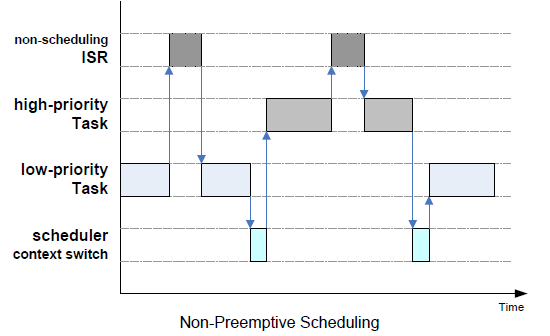
\includegraphics[width=0.4\textwidth]{images/Betriebssysteme/NonPreemptiveScheduling.png} \ \ \ \ \ \ \ \ \ \
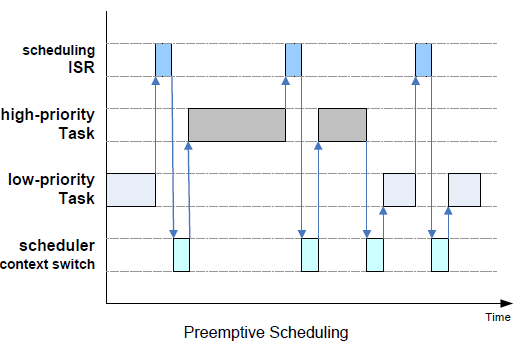
\includegraphics[width=0.4\textwidth]{images/Betriebssysteme/PreemptiveScheduling.png}
\end{multicols}
\textbf{Ziele:}
\begin{itemize}
    \item Hohe CPU Auslastung (Ideal 100\%, Normal 40-90\%)
    \item Hoher Durchsatz (Zahl der Tasks pro Zeiteinheit)
    \item Faire Behandlung der Tasks (im Mittel gleicher CPU-Zeitanteil für jeden Benutzer)
    \item Ausführungszeit: Zeitspanne vom Jobbeginn bis Jobende.
    \item Kurze Wartezeit: Der Scheduler kann nur die Wartezeiten in den Waiting- und ssen beeinflussen.
    \item Kurze Antwortzeit (vom Jobstart bis eine erste Reaktion an den Bediener erfolgen kann): Der Benutzer empfindet es als besonders unangenehm, wenn eine Reaktion des Systems lange ausbleibt.
\end{itemize}

\subsubsection{Scheduling Strategien}
\textbf{Cooperative scheduling:} Jeder Prozess läuft solange, bis er die CPU selber freigibt. Dieses einfache Verfahren erlaubt einen minimalen Verwaltungsaufwand. Es funktioniert
nur solange, bis ein Prozess die CPU nicht mehr abgibt (fehlende Fairness). Die Reaktionszeiten hängen direkt von den durch die Prozesse belegten Laufzeiten ab.\\ \\
\textbf{Round-robin scheduling (Zeitschiebeverfahren):} Es wird versucht, die Rechenzeit möglichst gleichmässig auf alle lauffähigen Prozesse zu verteilen. Zu diesem Zweck bildet das OS gleichmässige Zeitschlitze (Quantum) mit Hilfe eines Hardware-Zeitgebers (Timer). Jeweils nach Ablauf einer Zeitscheibe (Tick) wird der alte Prozess zuhinterst in der sse eingetragen und der neue Prozess zuvorderst der Liste entnommen. Somit geht man bei diesem Verfahren davon aus, dass alle Prozesse zu jedem Zeitpunkt gleich wichtig sind. \\ \\
\textbf{Priority based scheduling:}
Jedem Prozess wird vom Anwender eine Priorität zugewiesen. Derjenige mit der höchsten Priorität in der sse erhält den Prozessor zugeteilt. Damit nicht wie beim cooperative scheduling ein einzelner Prozess die CPU monopolisieren kann, wird in regelmässigen Zeitabständen die sse geprüft, ob Prozesse mit der gleichen oder einer höheren Priorität vorhanden sind. Ist das der Fall, so findet unter diesen Prozessen eine nach dem Round-Robin wechselnde Zuteilung statt. \\ \\
\textbf{Preemptive scheduling:}
Jedem Prozess wird vom Anwender eine Priorität zugewiesen. Derjenige mit der höchsten Priorität in der sse erhält den Prozessor zugeteilt. Wird durch ein Ereignis ein Prozess mit höherer Priorität als der ablaufende Prozess lauffähig, so findet augenblicklich eine Neuzuteilung statt. Der laufende Prozess wird also zugunsten des wichtigeren Prozesses verdrängt. 


\subsection{Interprozess-Kommunikation}
Sind die einzelnen Prozesse voneinander unabhängig, wie dies z.B. bei Applikationen
auf einem Arbeitsplatzrechner meist der Fall ist, so ist eine Abstimmung
zumindest bei den gemeinsamen Betriebsmitteln nötig. Wird eine grössere Applikation in mehrere Prozesse aufgeteilt, so besteht ein höherer
Kommunikationsbedarf. Dies kann ein gegenseitigs Synchronisieren im Zeitablauf
sein oder auch das Weiterreichen von Verarbeitungsdaten.

\subsubsection{Problem der Ressourcenteilung}
In der Parallelverarbeitung finden Zugriffe von mehreren Tasks auf gemeinsame
Betriebsmittel statt:
\begin{itemize}
    \item Gemeinsame Datenstrukturen (shared data structures)
    \item Gemeinsam benutzte Dateien (shared files)
    \item Gemeinsam benutzte Hardware (shared hardware)
\end{itemize}
Solche gleichzeitige Zugriffe auf gemeinsame Betriebsmittel ergeben aber Probleme. Die Ursache solcher Probleme ist der unkoordinierte, parallele Programmablauf, im Einzelcomputersystem durch das Rescheduling erzeugt, welches
zwischen zwei beliebigen Assembleranweisungen (Maschineninstruktionen) stattfinden kann. Die Zugriffe auf gemeinsame Mittel werden \textbf{kritische Bereiche oder Regionen}
genannt. Zur Lösung des Problems ist ein wechselseitiger Ausschluss (\textbf{mutual exclusion})
der Zugriffsoperationen notwendig.
Die Grundelemente für den wechselseitigen Ausschluss sind \textbf{Semaphoren}. Es handelt sich um spezielle Objekte im Betriebssystem.
Eine weitere Möglichkeit der Absicherung kann durch Koordination mittels
Meldungen erfolgen.

\subsubsection{Semaphoren}
Bei einem Semaphor handelt sich dabei um ein Betriebssystem-Objekt für die Absicherung und Synchronisation von Prozessen. Es besteht aus einem Zähler und einer Warteschlange für die Aufnahme blockierter Prozesse. Die Nutzungsoperationen wurden von Dijkstra mit P (proberen, prüfen) und V (verhogen, erhöhen) bezeichnet.\\ \\
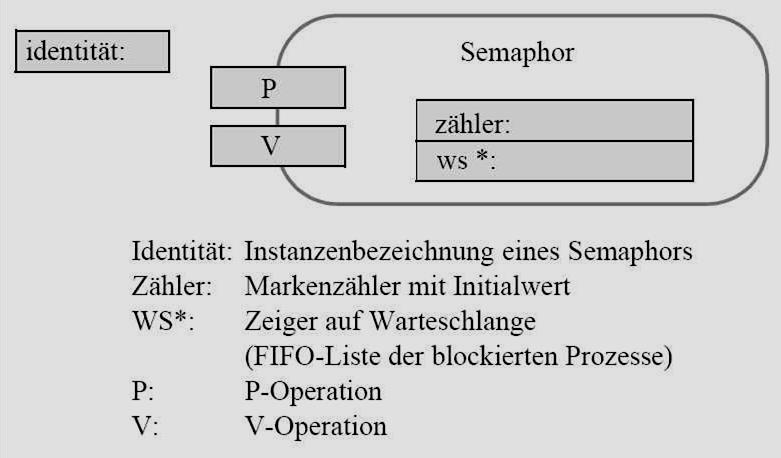
\includegraphics[width=0.4\textwidth]{images/Betriebssysteme/Semaphor.png}\ \ \
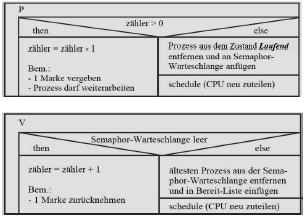
\includegraphics[width=0.35\textwidth]{images/Betriebssysteme/PVOperation.png}\\\\
Bei einem Aufruf der P-Operation (vor Eintritt in den kritischen Bereich) wird der Zähler dekrementiert. Ist der Zähler danach grösser gleich 0, so setzt der Prozess seine Aktionen fort. Ist der Zähler jedoch kleiner als 0, kehrt der Kontrollfluss nicht aus der Operation zurück. Der aufrufende Prozess wird blockiert und in die Warteschlange des Semaphors eingereiht. Bei einem Aufruf der V-Operation (beim Austritt aus dem kritischem Bereich) wird der Zähler inkrementiert. Es wird ein Prozess aus der Warteschlange entnommen und entblockiert, falls die Warteschlange nicht leer ist. Der entblockierte Prozess setzt dann seine Aktionen mit denen fort, die dem P-Aufruf folgen, der den Prozess blockierte. Die hier erläuterte Funktionsweise der Semaphoroperationen erlaubt eine einfache Ermittlung, ob es Prozesse gibt, die am Semaphor blockiert sind: ist der Semaphorzähler kleiner als 0, so gibt es noch blockierte Prozesse.\\\\
\textbf{Binäre Semaphore vs. Zählende Semaphore:}
Semaphore, deren Zähler aufgrund der Initialisierung und der Verwendung eine "'1"' als grössten positiven Wert annehmen können, werden oftmals auch binäre Semaphore bzw. Mutex locks bezeichnet. Semaphore, deren Zähler grössere positive Werte als "'1"' annehmen können, werden zählende Semaphore genannt.\\\\
\textbf{Semaphore mit Prioritätenvererbung:} Besitzt ein Task niedriger Priorität (T1) eine Semaphore, so kann es passieren, dass ein Task hoher Priorität (T2) nicht weiterlaufen kann, weil dieser den gleichen Semaphore belegen möchte, dieser aber bereits von T1 belegt ist. Die Priorität des Prozesses T1 wird deshalb temporär auf jene von T2 erhöht (bis die Semaphore-Marke zurückgegeben).\\\\
\textbf{Vorgehen für die Synchronisation von Prozessabläufen:} Zuerst den Semaphor mit 0 initialisieren. Danach in einem Prozess mit der P-Operation auf eine "'Marke"' warten. Im anderen Prozess mit der V-Operation eine "'Marke"' erzeugen bzw. weitergeben. Bei einer einfachen Synchronisation muss Task1 eventuell auf Task 2 warten, umgekehrt aber nicht (nicht symmetrisch). Bei einer wechselseitigen Synchronisation von mehreren Tasks muss eine zweifache Synchronisation vorgenommen werden, damit nicht einzelne Tasks vorauseilen können. 

\subsubsection{Weiterführende Konzepte}
\begin{minipage}{0.5\textwidth}
    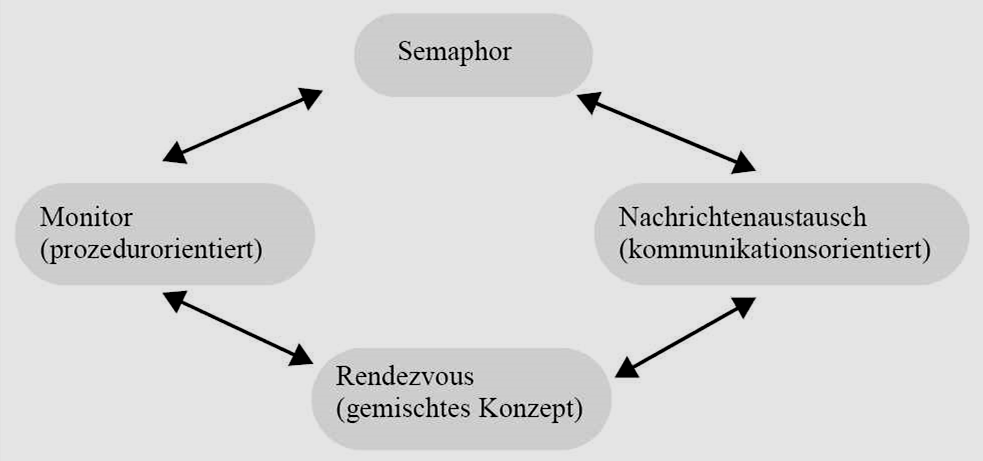
\includegraphics[width=0.8\textwidth]{images/Betriebssysteme/KonzepteInterprozesskommunikation.png}
\end{minipage}
\hfill
\begin{minipage}{0.45\textwidth}
    Jedes dieser Konzepte weist bezüglich einer bestimmten Problemklasse seine Vorzüge auf. Wesentlich ist jedoch, dass alle Konzepte funktional äquivalent sind, d.h. jedes Konzept kann in seiner Wirkungsweise durch jedes andere nachgebildet werden.
\end{minipage}

\subsubsection{Nachrichtenaustausch}
Die Interprozess-Kommunikation lässt sich auch mittels Meldungen realisieren, die über softwaremässige Briefkästen (mailboxes) versandt und empfangen werden. Das Konzept funktioniert sinngemäss wie die Briefpost.\\\\
\textbf{Mailbox:} Kann eine maximale Anzahl von Meldungen aufnehmen (beim Kreieren
der Mailbox festgelegt).
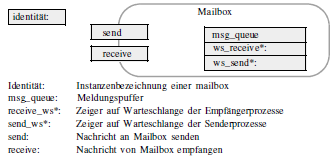
\includegraphics[width=0.5\textwidth]{images/Betriebssysteme/Mailbox.png}\\\\
\textbf{Message:} Variable Meldungslänge; die Maximallänge wird beim Erzeugen der Mailbox
festgelegt. Es befindet sich kein Absender auf dem Umschlag. Jeder Prozess kann aus jeder Mailbox eine Meldung holen.\\\\
\textbf{Senden einer Meldung:}
Wenn der Empfänger wartet, dann wird die Nachricht direkt an ihn weitergereicht. Der Empfängerprozess wechselt damit vom Zustand '"wartend'" in den Zustand '"bereit'". Wenn kein Empfänger wartet, dann wird die Nachricht in der Mailbox abgelegt. Ist die Mailbox bereits voll (maximale Anzahl an Meldungen gespeichert),
so muss der sendende Prozess auf das Ablegen warten. Dieses Warten kann je nach Betriebssystem mit einer Zeitlimite (timeout) belegt werden. Unterstützt das Betriebssystem Meldungsprioritäten, so wird die Meldung
entsprechend ihrer Priorität eingeordnet.\\\\
\textbf{Empfangen einer Meldung:} Wenn keine Meldung in der Mailbox bereit liegt, so muss der Prozess warten. Dieses Warten kann je nach Betriebssystem mit einer Zeitlimite (timeout) belegt werden. Der blockierte Prozess kommt je nach den unterstützten Möglichkeiten entweder an das Ende der Warteschlange (FIFO-Verfahren) oder wird entsprechend seiner Priorität (Prioritäts-verfahren) in die Warteschlange eingereiht.

\subsection{Deadlock}
Ein Deadlock ist eine Situation, in welcher mehrere Threads eines Systemes permanent geblockt sind, weil Ressourcen Anforderungen nicht erfüllt werden können.

\subsubsection{Bedingungen für das Auftreten}
\begin{itemize}
    \item \textbf{Mutual Exclusion:} Auf eine Ressource kann nur von jeweils einem Task zugegriffen werden.
    \item \textbf{No Preemption:} Eine nicht preemptive Ressource kann nicht dem Task entzogen werden, welcher momentan auf sie zugreift. Sie ist nur verfügbar wenn der zugreifende Task sie wieder freigibt.
    \item \textbf{Hold and Wait:} Ein Task besitzt bereits gewisse Ressourcen, benötigt aber noch weitere um fortzufahren.
    \item \textbf{Circular Wait:} Eine Kette von zwei oder mehr Task existiert, wenn jeder Task eine Ressource besitzt, welche vom nächsten Task der Kette angefordert wird.
\end{itemize}

\subsubsection{Beispiele}
\begin{multicols}{2}
    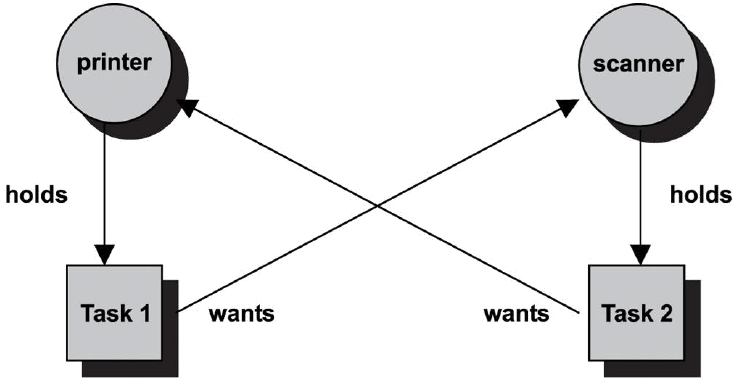
\includegraphics[width=0.5\textwidth]{images/Betriebssysteme/deadlock_2.png}
    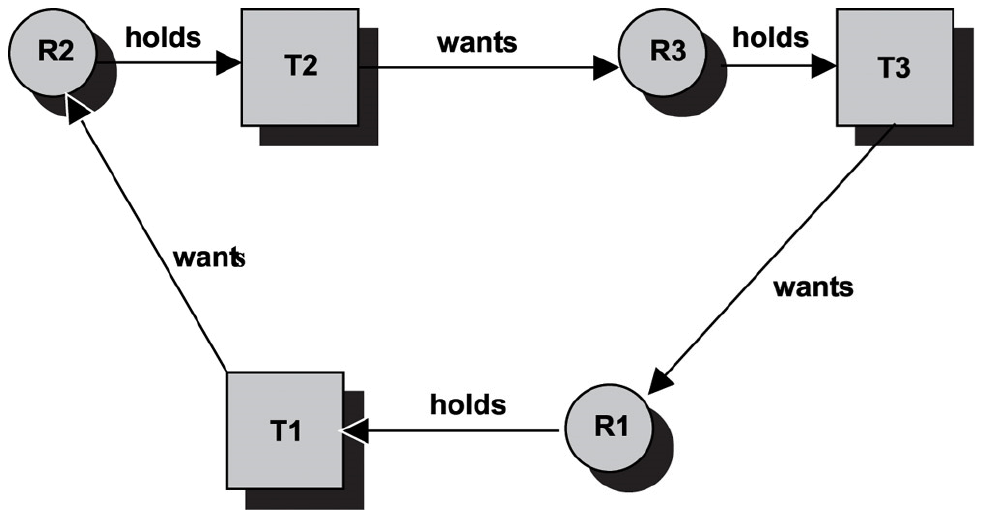
\includegraphics[width=0.5\textwidth]{images/Betriebssysteme/deadlock_3.png}
\end{multicols}

\subsubsection{Erkennung von Deadlocks mit einem Prozessfahrplan}
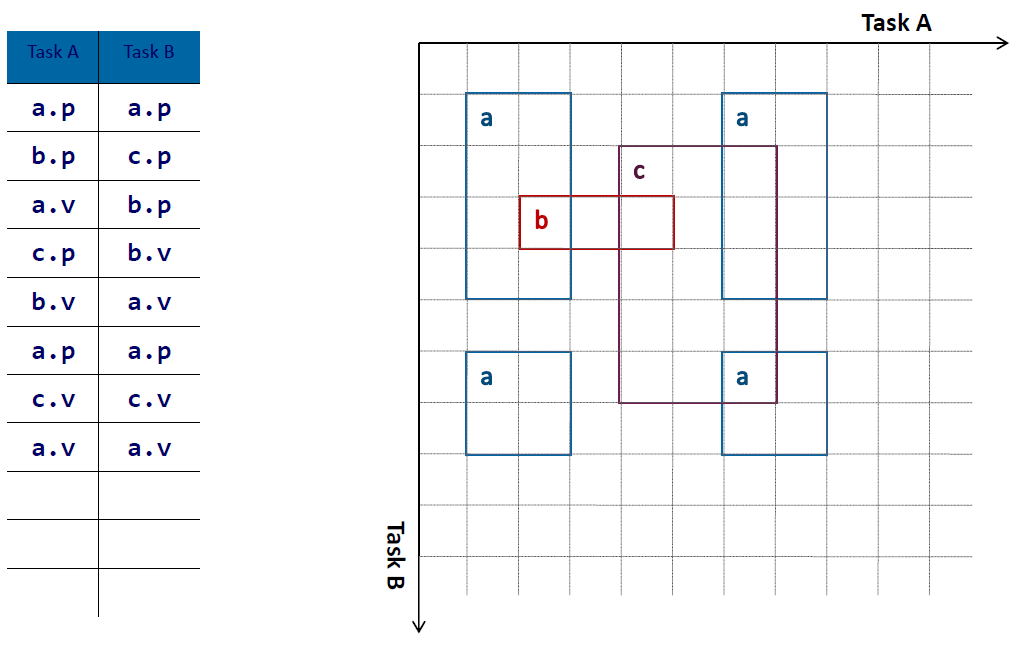
\includegraphics[width=0.6\textwidth]{images/Betriebssysteme/fahrplan.png} \\
\textbf{Wichtig:} Es müssen immer alle Prozesse gemeinsam angeschaut werden. 


\subsubsection{Verhinderung}
\begin{itemize}
    \item \textbf{Eliminieren des Hold and Wait:} Ein Task fordert zu einem Zeitpunkt alle Ressourcen an, welche dieser benötigt und kann nur beginnen, wenn er alle Ressourcen erhalten hat.
    \item \textbf{Eliminieren des No Preemption:} Ein Task muss bereits erhaltene Ressourcen wieder freigeben, wenn eine benötigte Ressource nicht erhalten wurde. Der Task muss dann wiederum alle Ressourcen anfordern.
    \item \textbf{Eliminieren des Circular Wait:} Alle Task müssen die Ressourcen in der selben Reihenfolge anfordern.
\end{itemize}

\subsection{Priority Inversion}
In einem Prioritäten basierten System werden höher priorisierte Task vor den niedrigeren priorisierten Task abgearbeitet. Wenn nun ein hoch priorisierter Task auf eine Ressource eines niedrig priorisierten Tasks warten muss, so ist das eine Priority Inversion.

\subsubsection{Bounded Priority Inversion}
Situation: Ein hoch priorisierter Task teilt eine Ressource mit einem niedrig priorisierten Task. Der hoch priorisierte Task muss nun warten, bis der niederig priorisierte Task die Ressource freigibt. \\
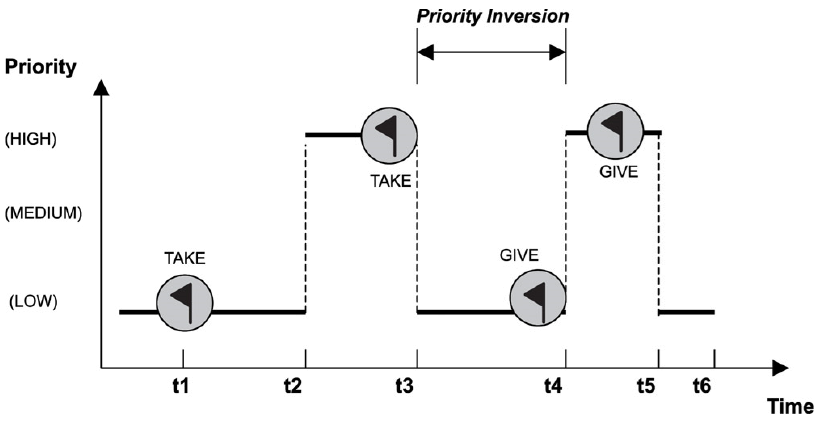
\includegraphics[width=0.5\textwidth]{images/Betriebssysteme/bounded_priority.png}

\subsubsection{Unbounded Priority Inversion}
Situation: Ein hoch priorisierter Task teilt eine Ressource mit einem niedrig priorisierten Task. Die Zeit, welche der niedrig priorisierte Task die Ressource benötigt, ist bekannt. Es ist nun möglich das ein mittel priorisierter Task den niedrig priorisierten Task unterbricht für eine unbestimmte Zeit, was dazu führt, dass der hoch priorisierte Task eine unendlich lange Zeit warten muss. \\
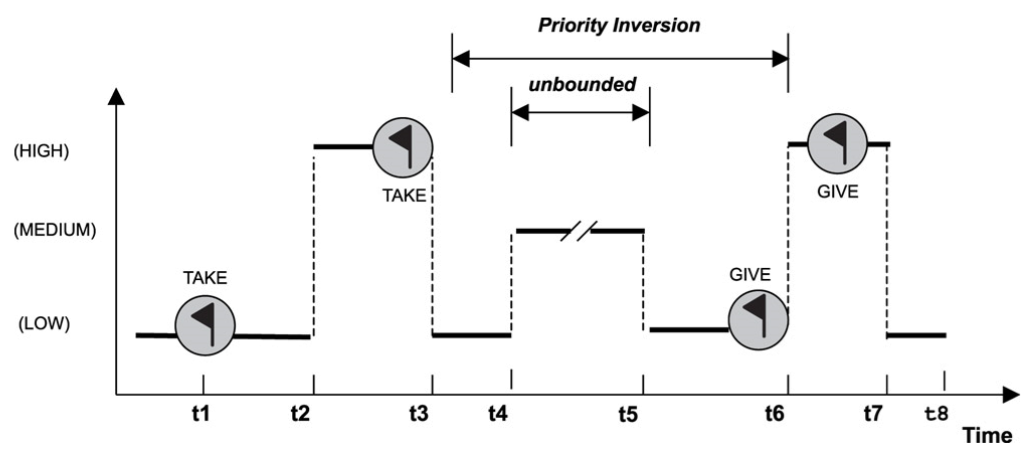
\includegraphics[width=0.5\textwidth]{images/Betriebssysteme/unbounded_priority.png}

\subsubsection{Priority Inheritance Protocol}
Das Priority Inheritance Protocol ist ein Protokoll, welches die Priorität eines Tasks erhöht, wenn eine Ressource dieses Tasks von einem höher priorisierten Tasks angefordert wird. Die Priorität wird auf die selbe Priorität wie diejenige des hoch priorisierten Tasks erhöht. \\
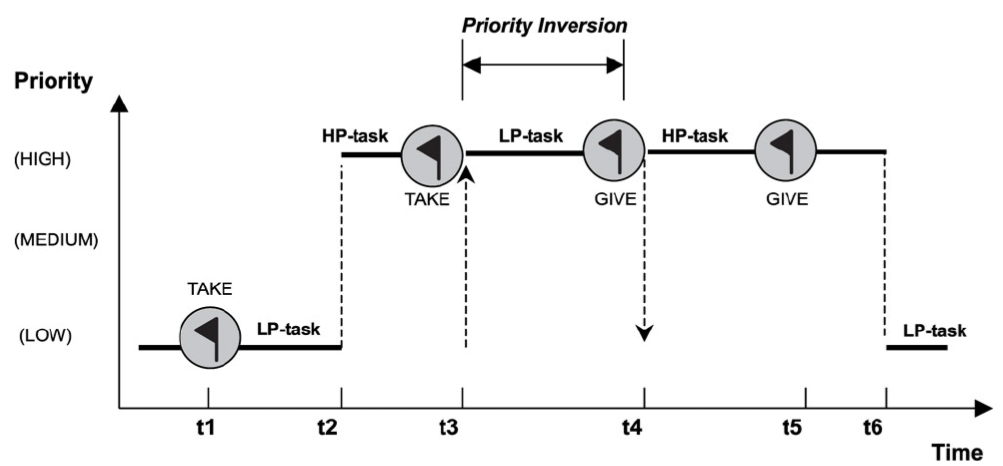
\includegraphics[width=0.5\textwidth]{images/Betriebssysteme/priority_inheritance.png}

\subsubsection{Ceiling Priority Protocol}
Im Ceiling Priority Protocol ist die Priorität jedes Tasks bekannt. Ebenfalls sind alle Ressourcen eines Tasks bekannt und somit die höchstmögliche Priorität pro Ressource. Die Tasks werden mit diesem Protokoll automatisch auf die höchstmögliche Priorität angehoben. Deadlocks können mit diesem Protokoll nie auftreten.

\subsection{Real-Time Operating System (RTOS)}
Die meisten RTOS beeinhalten folgende Komponenten:
\begin{itemize}
    \item Scheduler
    \begin{itemize}
        \item Wird von jedem Kernel beeinhaltet und folgt einem Algorithmus, welcher definiert welcher Task wann ausgeführt wird.
        \item Einige Beispiele für Algorithmen sind Round Robin und Preemptive Scheduling.
    \end{itemize}
    \item Objekt
    \begin{itemize}
        \item Objekte sind spezielle Kernel Konstrukte, welche helfen Anwendungen für Echtzeit Systeme zu erstellen.
        \item Einige Beispiele: Tasks, Semaphoren und Nachrichten.
    \end{itemize}
    \item Service
    \begin{itemize}
        \item Service sind Operationen, welche vom Kernel an Objekten durchgeführt werden.
        \item Einige Beispiele: Timing, Interrupt Handling und Ressourcen Management.
    \end{itemize}
\end{itemize}

\subsection{FreeRTOS}
\subsubsection{Vorteile}
\begin{itemize}
    \item Die Scheduling Variante kann gewählt werden: Preemptive oder Cooperative.
    \item Enthält einen Lowpowermode.
    \item Kleine Codegrösse, braucht im Schnitt 4K bis 9K.
    \item Support für über 30 verschiedene System Architekturen.
    \item Sehr gut portierbar, da der Code hauptsächlich in C geschrieben ist.
\end{itemize}

\subsubsection{Unterstütze Objekte}
Folgende Objekte werden unterstützt:
\begin{multicols}{2}
    \begin{itemize}
        \item Tasks
        \item Semaphoren (Binary, Counting und Recursive)
        \item Mutexes
        \item Queues
        \item Event Groups
        \item Queue Sets
        \item Software Timers
    \end{itemize}
\end{multicols}
RTOS Objekte können dynamisch oder in statisch alloziertem RAM angelegt werden.

\subsubsection{Task States}
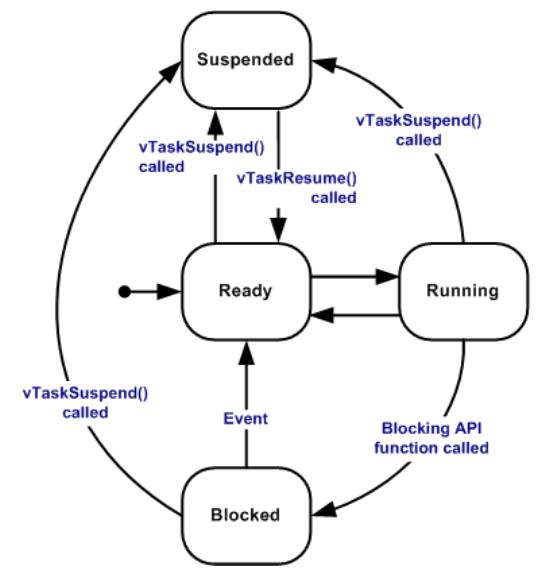
\includegraphics[width=0.4\textwidth]{images/Betriebssysteme/freertos_taskstates.png}\\
\textbf{Beispiel:}
\lstinputlisting[language=C]{code/freertos_taskmanagement.c}

\subsubsection{Semaphoren}
\textbf{Binary Semaphoren:} werden gebraucht für Mutual Exclusion und Synchronisationszwecke. \\
\textbf{Counting Semaphoren:} werden gebraucht für Zähl Events und Ressourcen Management. \\
\textbf{Mutex:} sind binäre Semaphoren, welche ein Prioritäts-Erbungs-System implementiert haben.

\subsubsection{Queues}
Queues sind die primäre Form von Kommunikation zwischen Tasks. Nachrichten können zwischen Tasks und zwischen Interrupts und Tasks gesendet werden. In den meisten Fällen sind Queues als FIFO ausgebaut. \\ \\
\textbf{Beispiel:}
\lstinputlisting[language=C]{code/freertos_queues.c}

\subsubsection{Event Groups}
Eine Event Gruppe ist ein zusammengehörende Gruppe von Event Bits. Individuelle Event bits in einer Event Gruppe werden über die Bit Nummer angesprochen.

\subsubsection{Queue Sets}
Queue Sets stellen einen Mechanismus zur Verfügung, welcher es einem RTOS Task erlaubt aktuelle Lesezugriffe auf mehrere Queues oder Semaphoren gleichzeitig zu blockieren. Ein Queue Set muss explizit erstellt werden. Anschliessend können Queues und Semaphoren zu einem Queue Set hinzugefügt werden. Die Queues und Semaphoren müssen jedoch leer sein beim Zeitpunkt des hinzufügens. \\ \\
\textbf{Beispiel:}
\lstinputlisting[language=C]{code/freertos_queueset.c}

\subsubsection{Software Timer}
Ein Software Timer erlaubt es eine Funktion zu einer gegebenen Zeit in der Zukunft auszuführen. Die Funktion welche vom Timer ausgeführt wird, heisst Callback Funktion. Die Zeit zwischen dem starten des Timers und dem ausführen der Callback Funktion wird Timer Periode genannt. \\ \\
\textbf{Beispiel:}\\
Timer 1: One-Shot Timer, Timer 2: Auto-Reload Timer \\
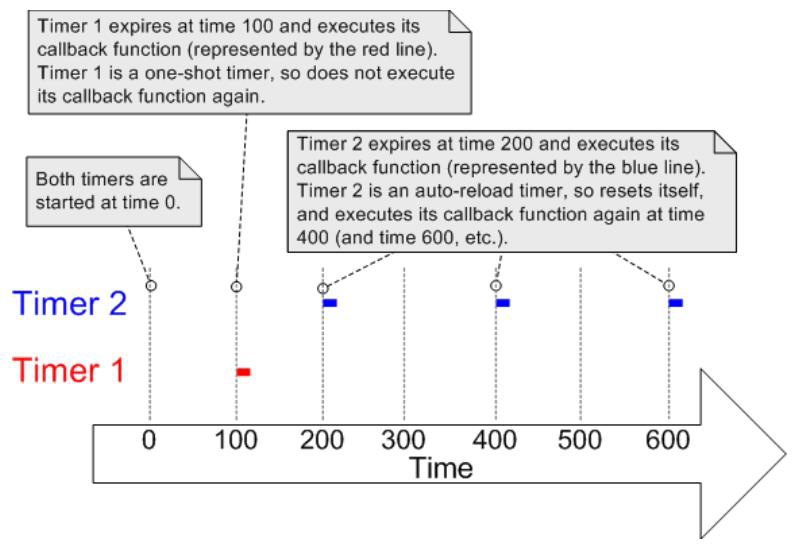
\includegraphics[width=0.6\textwidth]{images/Betriebssysteme/freertos_timer.png}